In high-stakes decision making, models must provide not only reliable predictions but also human-understandable explanations \cite{murdoch2019interpretable, doshi2017towards}. 
This has motivated \emph{interpretable-by-design} models, whose structure permits direct inspection of their behavior \cite{molnar2020interpretable}.
Interpretability, however, is not a yes-or-no property but a continuum: interpretable-by-design models range from more to less interpretable, and gains in predictive accuracy often come at the cost of greater structural complexity \cite{rudin2019stop, lipton2018mythos}.

\begin{figure*}[t]
  \centering
  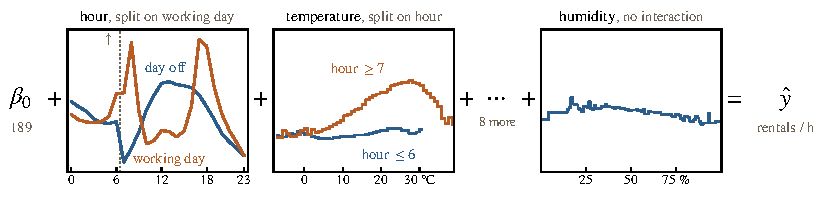
\includegraphics[width=\textwidth]{images/concept.pdf}
  \caption{A CALM fitted on the Bike Sharing dataset: the prediction sums one plot per feature, each plot holding one curve per region. The hour splits on the working day; the temperature splits on the hour, mattering by day and barely at night; the humidity interacts with no feature and keeps one curve. The dotted line on the hour's plot marks where the temperature's and the year's regions switch and its arrow gives the sign of the hidden jump; Section~\ref{subsec:interpretability-properties} explains it in depth.}
  \label{fig:concept-image}
\end{figure*}


This trade-off is evident in GAMs~\cite{lou2012intelligible} and their extension, \gamms~\cite{caruana2015intelligible}.
GAMs model the prediction as a sum of univariate effects, which makes them highly interpretable but blind to feature interactions which limits their accuracy.
\gamms~gain accuracy by adding selected pairwise interactions, but the interaction terms cost them two interpretability properties \cite{radenovic2022neural}:
(i) a prediction no longer splits into one contribution per feature, because an interaction term belongs to two features jointly, and
(ii)~global auditing is hard to do visually: a feature's effect is spread over its univariate and bivariate terms, so no single plot shows how the feature affects the prediction (see Section~\ref{subsec:interpretability-properties}).

We introduce \emph{Conditionally Additive Local Models (CALMs)}, a model class that narrows this trade-off: it stays close to GAMs in interpretability and close to \gamms~in accuracy.
The core idea is to learn \emph{conditional feature effects}: several univariate effects per feature, each active in a region of the input space where the feature is nearly additive, i.e., barely interacts with other features.
The regions are defined by threshold conditions on the features it interacts with.
Figure~\ref{fig:concept-image} shows a CALM fitted on the Bike Sharing dataset~\cite{fanaee2014event} and Figure~\ref{fig:hero} compares it with a GAM and a \gamm.

In this example, the feature \texttt{hour} interacts with \texttt{workingday}, so a CALM draws its effect as two curves, one for working and one for non-working days.
On working days rentals peak at the morning and evening commute, whereas on non-working days they rise to a single broad peak around midday.
The CALM thus captures the interaction while keeping (i) one contribution per feature and (ii) one plot per feature, unlike a GAM, which averages the two curves into one and loses accuracy, and a \gamm{}, which expresses the interaction as a pairwise surface and loses both interpretability properties.

\begin{figure*}[t]
  \centering
  \begin{subfigure}{0pt}\phantomsubcaption\label{fig:hero-gam}\end{subfigure}%
  \begin{subfigure}{0pt}\phantomsubcaption\label{fig:hero-calm}\end{subfigure}%
  \begin{subfigure}{0pt}\phantomsubcaption\label{fig:hero-ga2m}\end{subfigure}%
  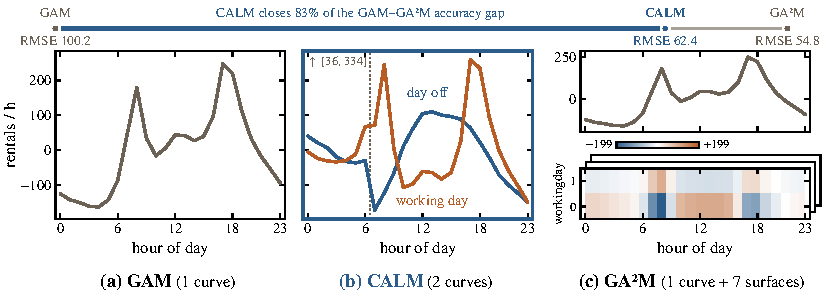
\includegraphics[width=\linewidth]{images/bike/hero}
  \caption{The effect of the hour on bike rentals (Bike Sharing dataset). Top: test RMSE (Table~\ref{tab:regr-rmse}); CALM closes 83\% of the gap from GAM to \gamm.
    (\subref{fig:hero-gam}) GAM: one curve. The interaction with the working day is averaged away, which limits accuracy.
    (\subref{fig:hero-calm}) CALM: one curve for working days and one for days off (at $d_{\max} = 1$). The dotted line mark a hidden jump (see Section~\ref{subsec:interpretability-properties} for more details).
    (\subref{fig:hero-ga2m}) \gamm: a curve and seven 2D surfaces (only one shown here) for decoding the effect of the hour, which limits its interpretability.}
  \label{fig:hero}
\end{figure*}


We fit CALMs with a three-step distillation pipeline:
(1) train a black-box reference model that captures the interactions in the data;
(2) for each feature, grow a CART-style tree~\cite{herbinger2022REPID} that splits the input space into regions of reduced interaction, then greedily keep the trees that matter most for reproducing the reference model's predictions;
(3) fit one curve per region with a region-aware backfitting.
Two parameters bound what a reader must inspect: the tree depth $d_{\max}$ caps how many curves each feature has and $K$ caps how many interactions the model captures in total.

\textbf{Contributions.}
(i) CALMs, an interpretable-by-design model class built on conditional feature effects (Section~\ref{subsec:model-overview});
(ii) a distillation-based training algorithm (Section~\ref{subsec:training});
(iii) a formal analysis showing that CALMs keep the two interpretability properties that \gamms~lose (Section~\ref{subsec:interpretability-properties});
(iv) an evaluation on 24 real-world regression and classification datasets, in which CALMs never lose to a GAM baseline and match or beat EB$^2$M on more than half (Section~\ref{sec:real-datasets});
(v) evidence that CALMs stay small and stable: about eight curves beyond a GAM, growing with tree depth as accuracy rises (Section~\ref{sec:complexity}), and the same structure for most features across resamples (Section~\ref{sec:stability});
(vi) a within-subjects user study ($N=25$), in which participants answered more accurately from CALM plots than from \gamm{} heatmaps (Section~\ref{sec:user-study}).
Code: \url{https://github.com/givasile/calm-paper}.
